\newpage
\section{Einleitung} \label{sec:Einleitung}
\subsection{Vorstellung des Projektes} \label{sec:Vorstellung des Projektes}
Im Projekt \textit{HeartRate2Go} geht es darum, mit einer App für eine Android Uhr die Herzfrequenz per Pulsoxymetrie zu messen und diese Messwerte in einer passenden GUI darzustellen. \\
Somit soll der Anwender bei der Kontrolle seines Pulses unterstützt werden und ihm einen guten, verständlichen Überblick bieten. Dies gilt sowohl für eine Ruhemessung, als auch für eine Messung während einer Aktivität. \\
\\
%Ablauf einer Messung, vllt mit Diagramm 
%Anwender trägt Uhr, startet App, wählt Messart aus, Messung startet, evtl Messung beenden, Abfrage über Stimmung, Smartphone zeigt Durchschnittswert an, Smartphone empfängt Daten automatisch von der Uhr, Smartphone zeigt Werte im Balkendiagramm an, GUI öffnen, GUI empfängt Messdaten per tcp über Smartphone (wird vom Smartphone gesteuert), Messdaten werden in GUI eingefügt und graphisch dargestellt, Messwerte können mit vergangen Messungen verglichen und auch gedruckt werden.
\textbf{Ablauf}\\
\\
Für die Nutzung für \textit{HeartRate2Go} sind drei Komponenten nötig:\\
\begin{itemize}
	\item Android-Uhr
	\item Android-Smartphone und
	\item Computer
\end{itemize}
Der Nutzer trägt die Android-Uhr am Handgelenk und startet auf dieser die \textit{HeartRate2Go-App}. Hier wird nun abgefragt, ob er eine Ruhemessung oder eine Aktivitätsmessung durchführen möchte. Anschließend wird die ausgewählte Messung durchgeführt. Bei einer Ruhemessung wird die Messung automatisch beendet, bei der Aktivitätsmessung muss der Benutzer die Messung manuell beenden. 
Nun wird der Anwender nach seiner Stimmung während der Pulsmessung gefragt, hier hat er die Auswahl zwischen gut, ok und schlecht. Außerdem wird der Durchschnittswert der soeben durchgeführten Messung gezeigt.\\
Die Übertragung der Messwerte von der Android-Uhr an das Android-Smartphone verläuft automatisch per Bluetooth. Auf der Smartphone-App werden die Messungen in einem Balkendiagramm angezeigt und bieten so einen ersten Überblick. \\
Nachdem das \textit{HeartRate2Go-Programm} auf einem Computer gestartet wurde, kann der Nutzer über die Smartphone-App die Übermittlung der Daten zu der GUI starten. Dort werden wird die neuste Messung und auch vergangene Messungen tabellarisch und grafisch dargestellt und zwischen den zwei Messtypen unterschieden. Des Weiteren ist auch ein Ausdrucken der Messwerte möglich.\\
\\
TODO: Ablaufdiagramm von Bö einfügen
\\  
\subsection{Medizinische Apps}\label{sec:Medizinische Apps}
Im Laufe der letzten Jahre wurde der Markt mit Apps, die einen medizinischen Hintergrund besitzen, überschüttet. Wenn man im deutschen iTunes-Store nach „Medizin“ sucht, erhält man mehrere hundert Einträge, dies gilt genauso für den Google-Play Store. \\
Im vergangen Jahr sind die Absatzzahlen von medizinischen Apps in Großbritannien, Frankreich, Niederlande und Deutschland um 42 Prozent gestiegen, vermeldet das GfK (Marktforschungszentrum).\\
Diese Apps decken nahezu jeden Bereich der Medizin ab, egal ob es um die Speicherung von Vitaldaten, die Messung von Vitaldaten mit einem zusätzlichen Messgerät und die Auswertung der Daten geht. Des Weiteren sind auch viele Nachschlagewerke darunter enthalten.\\
Zu beachten ist allerdings, dass keiner der Apps den Arztbesuch ersetzt. Sie geben lediglich eine erste Einschätzung und sind dadurch eine große Erleichterung für den Nutzer. Allerdings ist es auch so, dass jeder Programmierer eine App mit medizinischem Hintergrund in die verschiedenen Stores hochladen darf. Diese werde nicht auf ihren Nutzen hin überprüft, so sind auch viele Apps zu finden, die mehr als Spielerei gelten.\\
Kaum eine App ist ein Medizinprodukt nach dem Medizinproduktegesetzt, sie gelten lediglich als Wellness- beziehungsweise Lifestyle-Apps. \\
\\

\textbf{} 
%Thema und Zielsetzung: Stellen Sie zunächst Thema und Zielstellung der Arbeit vor.
%Theorie: Vermitteln Sie Ihre Theorie(n) über das Thema und geben Sie an, auf was sich Ihre Theorie stützt.
%Fragestellung: Teilen Sie mit, welche Fragen in der folgenden Arbeit beantwortet werden.
%Quellen: Welche Quellen haben Sie für Ihre Arbeit genutzt bzw. wie haben Sie Ihre Frage(n) beantwortet?
%Ergebnis: Führen Sie Ihre Ergebnisse auf, also teilen Sie mit, was Sie herausgefunden haben.
%Fazit: Stellen Sie am Ende des Abstracts eine Quintessenz auf. Sie können Ihr Fazit auch mit einer %Zukunftsprognose verbinden.

\subsection{Medizinische Kenntnisse - Pulsoxymetrie} 
Für die Messung des peripheren Pulses per Android-Uhr wird das Prinzip der Reflexions-Pulsoxymetrie genutzt. \\
Dieses Verfahren benötigt zwei Sensoren: zum einen eine Lichtquelle, zum anderen ein Lichtsensor. Die Lichtquelle sendet Infrarot-Lichtwellen aus, die durch die Haut dringen. Der Sensor misst die Lichtanteile, die absorbiert wurden. \\
Die Lichtabsorption im Blut ist abhänig von der Hämoglobinkonzentration und der Sättigung des Hämoglobins mit Sauerstoff. Oxigeniertes und desoxigeniertes Hämoglobin schwächen das Licht jeweils charakteristisch ab. \\
Mit diesem Prinzip ist es auch möglich, die Sauerstoffsättigung im kapillären Blut gemessen werden.\\
\\
\begin{center}
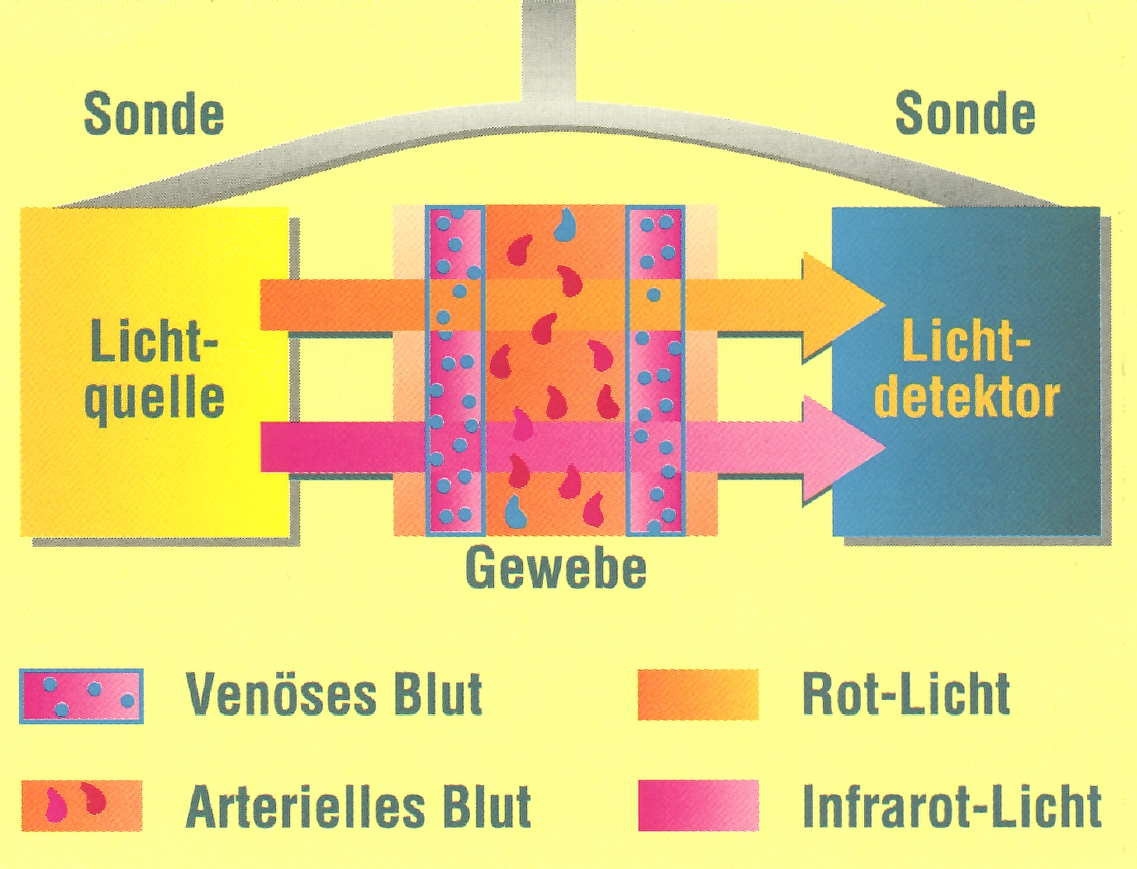
\includegraphics[scale=1.0]{images/pulsoxy.jpg} \\ 
Quelle: www.edoc.hu-berlin.de\\

\end{center}




% Kurze Erklärung 
% reicht das oder noch mehr?
TODO:
bitte Korrektur lesen
Quelle einfügen
Quelle: Behandlungsassistenz „… in der Arztpraxis“ von Dr. Uta Groger, Cornelsen Verlag, 1. Auflage, 2007



